Калориметрическая система детектора ATLAS имеет ключевую роль в измерении энергии и положения электронов, фотонов и заряженных адронов. Система калориметров является составной и состоит из четырёх основных частей \parencite{tdr_green} (рис. \ref{fig:atlas_cal}):
\begin {itemize}
    \item электромагнитная цилиндрическая;
    \item электромагнитная торцевая;
    \item адронная торцевая;
    \item форвард калориметр.
\end{itemize}\par
\begin{figure}[ht]
    \centering
    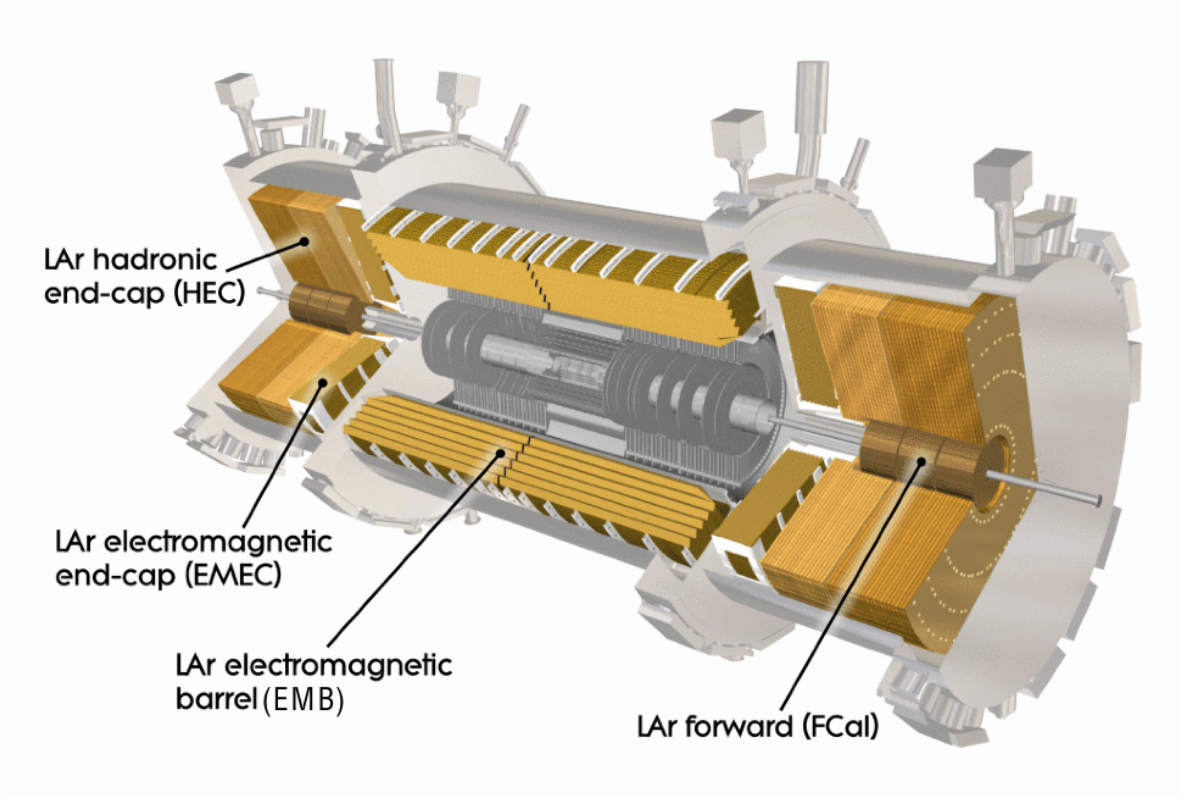
\includegraphics[width=0.8\linewidth]{atlas_cal.png}
    \caption{Схема калориметрической системы ATLAS}
    \label{fig:atlas_cal}
\end{figure}
Важной характеристикой системы калориметров является диапазон покрытия псевдобыстроты $|\eta|$. Эта величина показывает насколько направление движения элементарной частицы отличается от оси пучка и определяется как:
\begin{equation}
    \eta = -\ln(\tan(\frac{\Theta}{2})),
\end{equation}\par
где $\Theta$ -- угол между направлением импульса частицы и осью пучка. В физике коллайдеров зачастую используют именно этот показатель вместо простого полярного угла $\Theta$ в силу той особенности, что плотность числа рождённых частиц приблизительно постоянна в единицу $|\eta|$. По этой причине калориметры обычно сегментируют по псевдобыстроте, а не по телесному углу. Калориметрическая система ATLAS охватывает диапазон $|\eta|$ до 4.9.

\subsubsection{Электромагнитный калориметр}
Для прецизионного детектирования и измерения электронов и фотонов калориметрическая система ATLAS включает в себя электромагнитный калориметр. Он состоит из центрального (баррельного) блока (EMB -- electromagnetic barrel), покрывающего диапазон псевдобыстрот $|\eta| < 1,475$, и пары торцевых частей (EMEC -- electromagnetic end-cap), соответствующих области $1,375 < |\eta| < 3,2$. Электромагнитные калориметры ATLAS построены по гетерогенному принципу, то есть в них разделены функции поглощения и детектирования. В качестве активного вещества служит жидкий аргон, находящийся при температуре около 90K, а для поглощающего материала используется свинец. Между пластинами поглотителя также располагаются медно-каптоновые электроды, по которым происходит снятие сигнала.\par
Заряженная частица, попадая в калориметр, порождает в нём электромагнитный ливень (рис. \ref{fig:em_shower})\parencite{em_shower_wiki}, который детектируется по принципу ионизационной камеры: под воздействием электрического поля между заземлённым поглотителем и электродом, находящимся под высоким напряжением, ионы и электроны дрейфуют, причём последние индуцируют треугольный импульс на электроде(рис. \ref{fig:tri_impulse})(в действительности, сигнал является более сложным, чем просто треугольник -- в силу поглощения электронов загрязняющими примесями в активном веществе, такими как кислород или хлор, результирующий сигнал падает, а его форма домножается на небольшую экспоненту). Высота индуцированного импульса пропорциональна энергии, накопленной в ячейке калориметра. Время пика импульса используется для определения времени появления частицы.\par
\begin{figure}[ht]
    \centering
    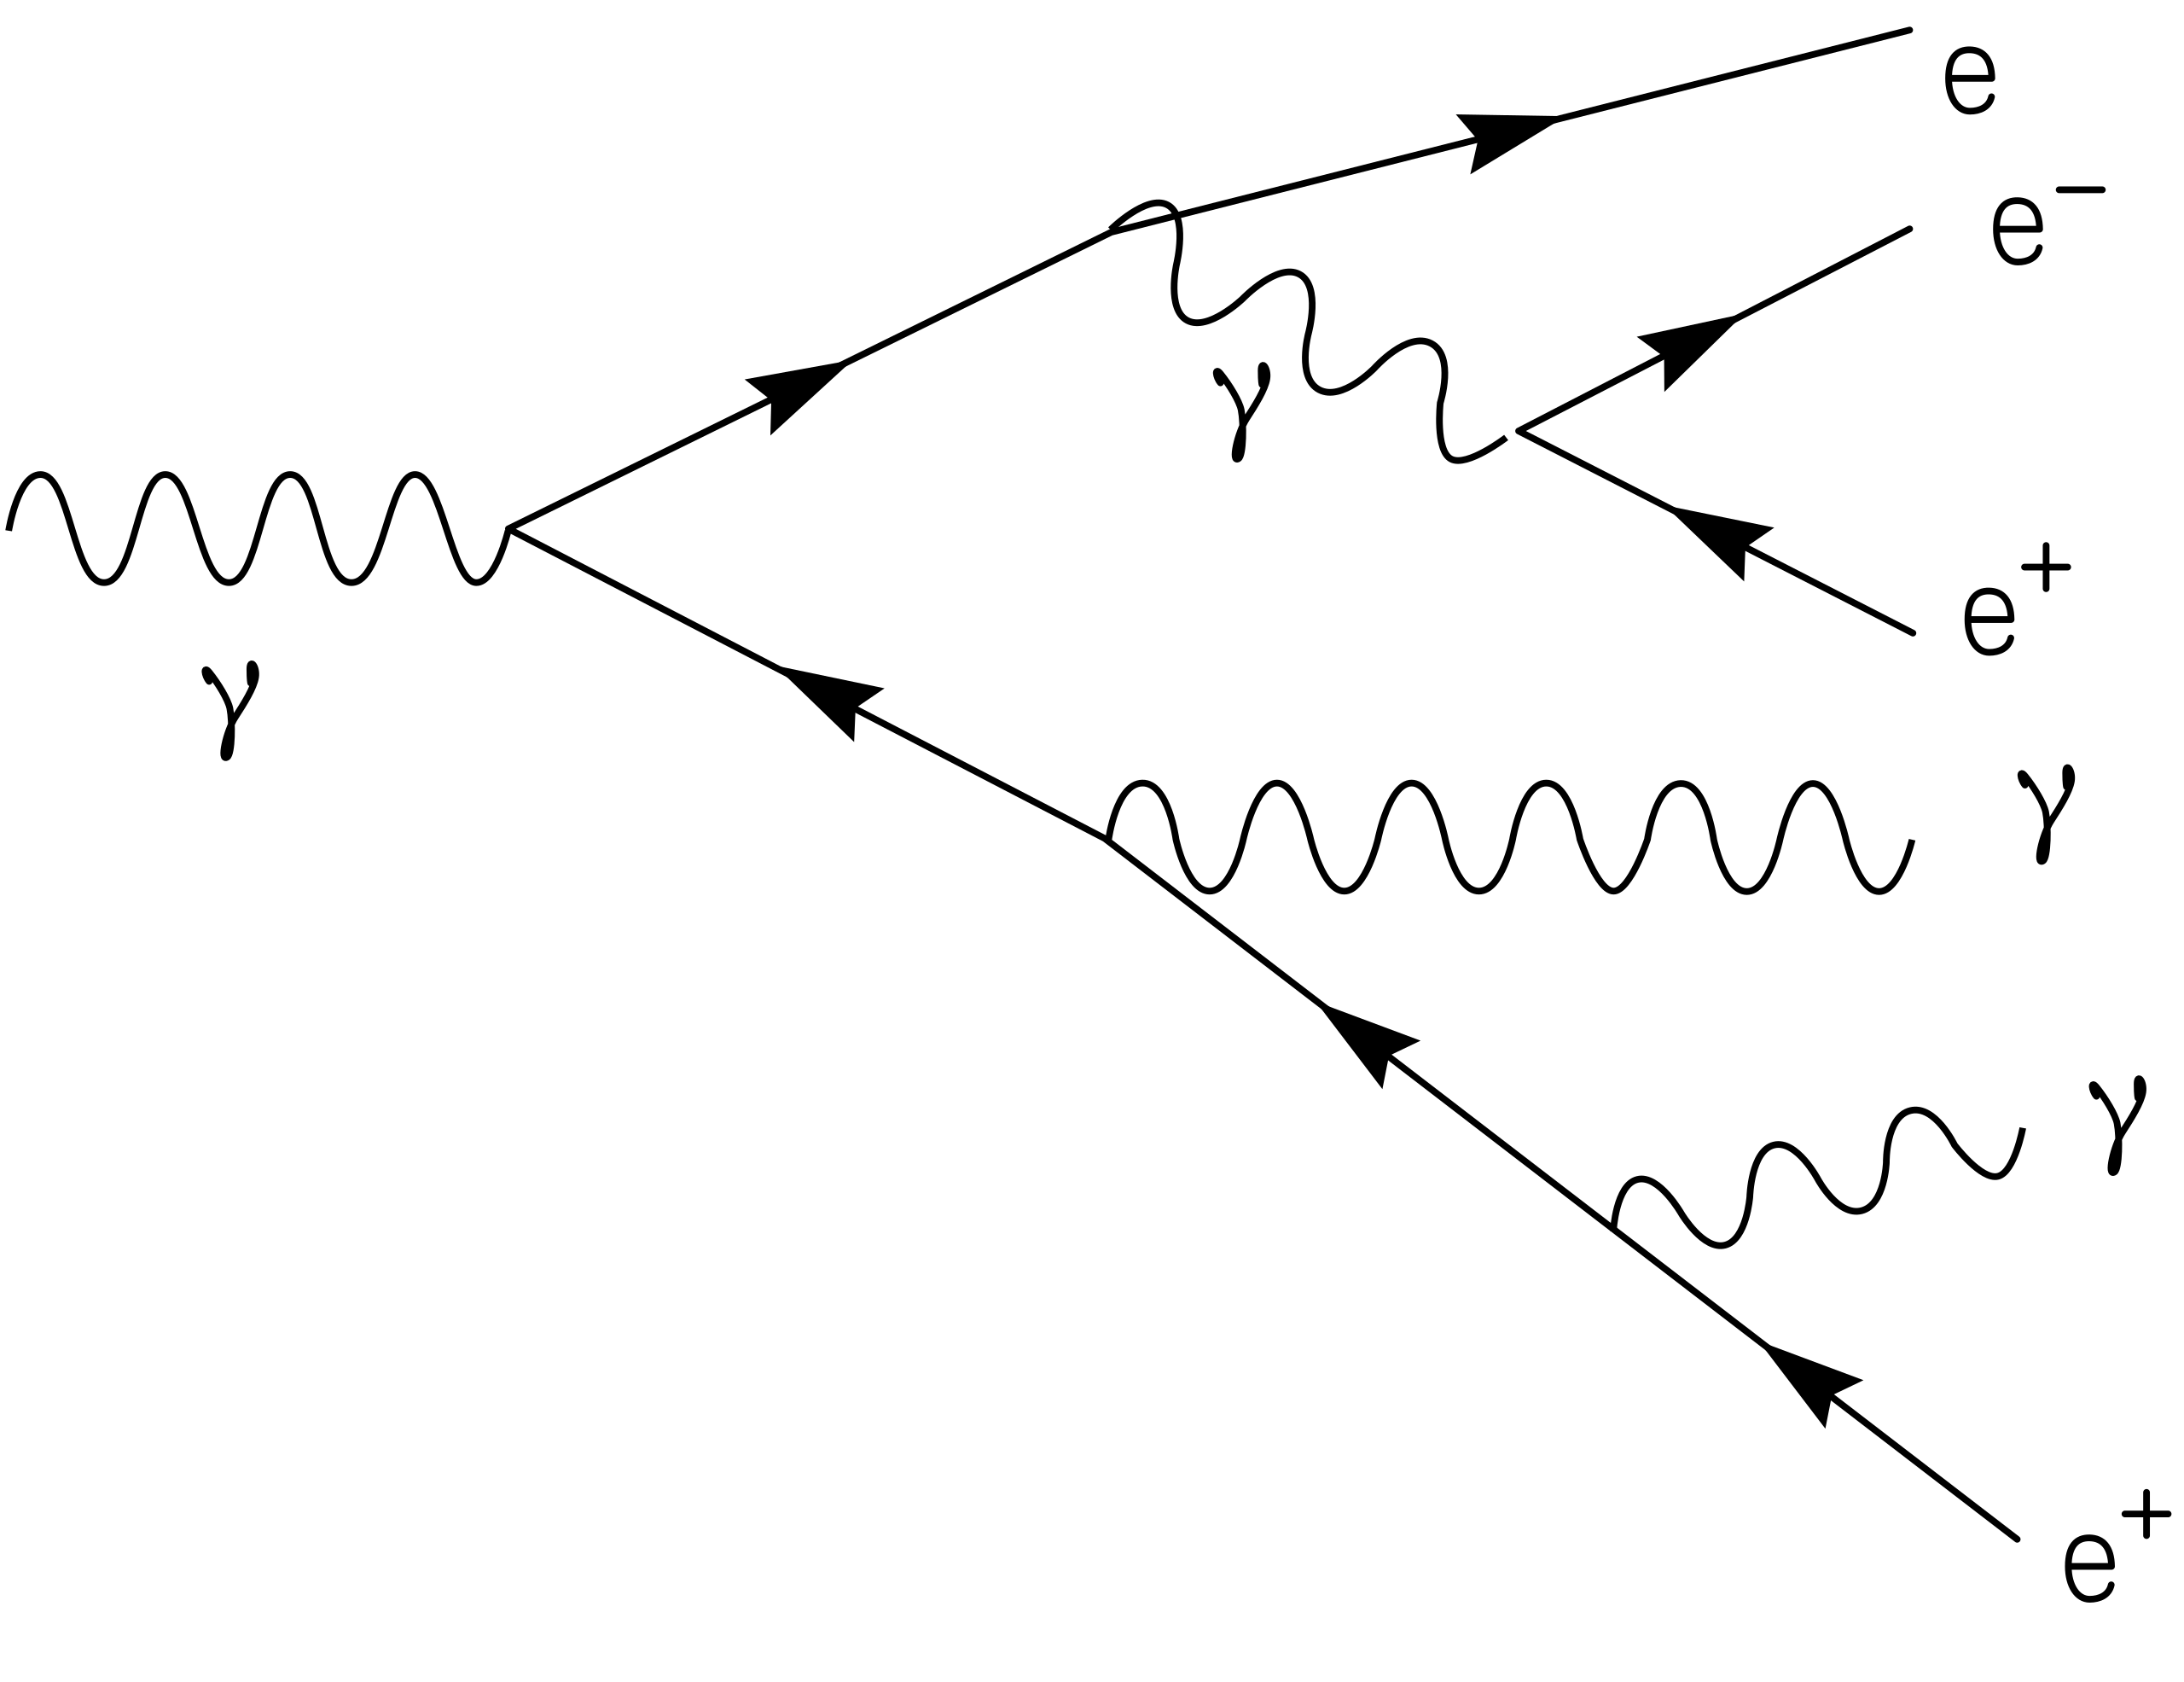
\includegraphics[width=0.5\linewidth]{em_shower.png}
    \caption{Схема электромагнитного ливня}
    \label{fig:em_shower}
\end{figure}
\begin{figure}[ht]
    \centering
    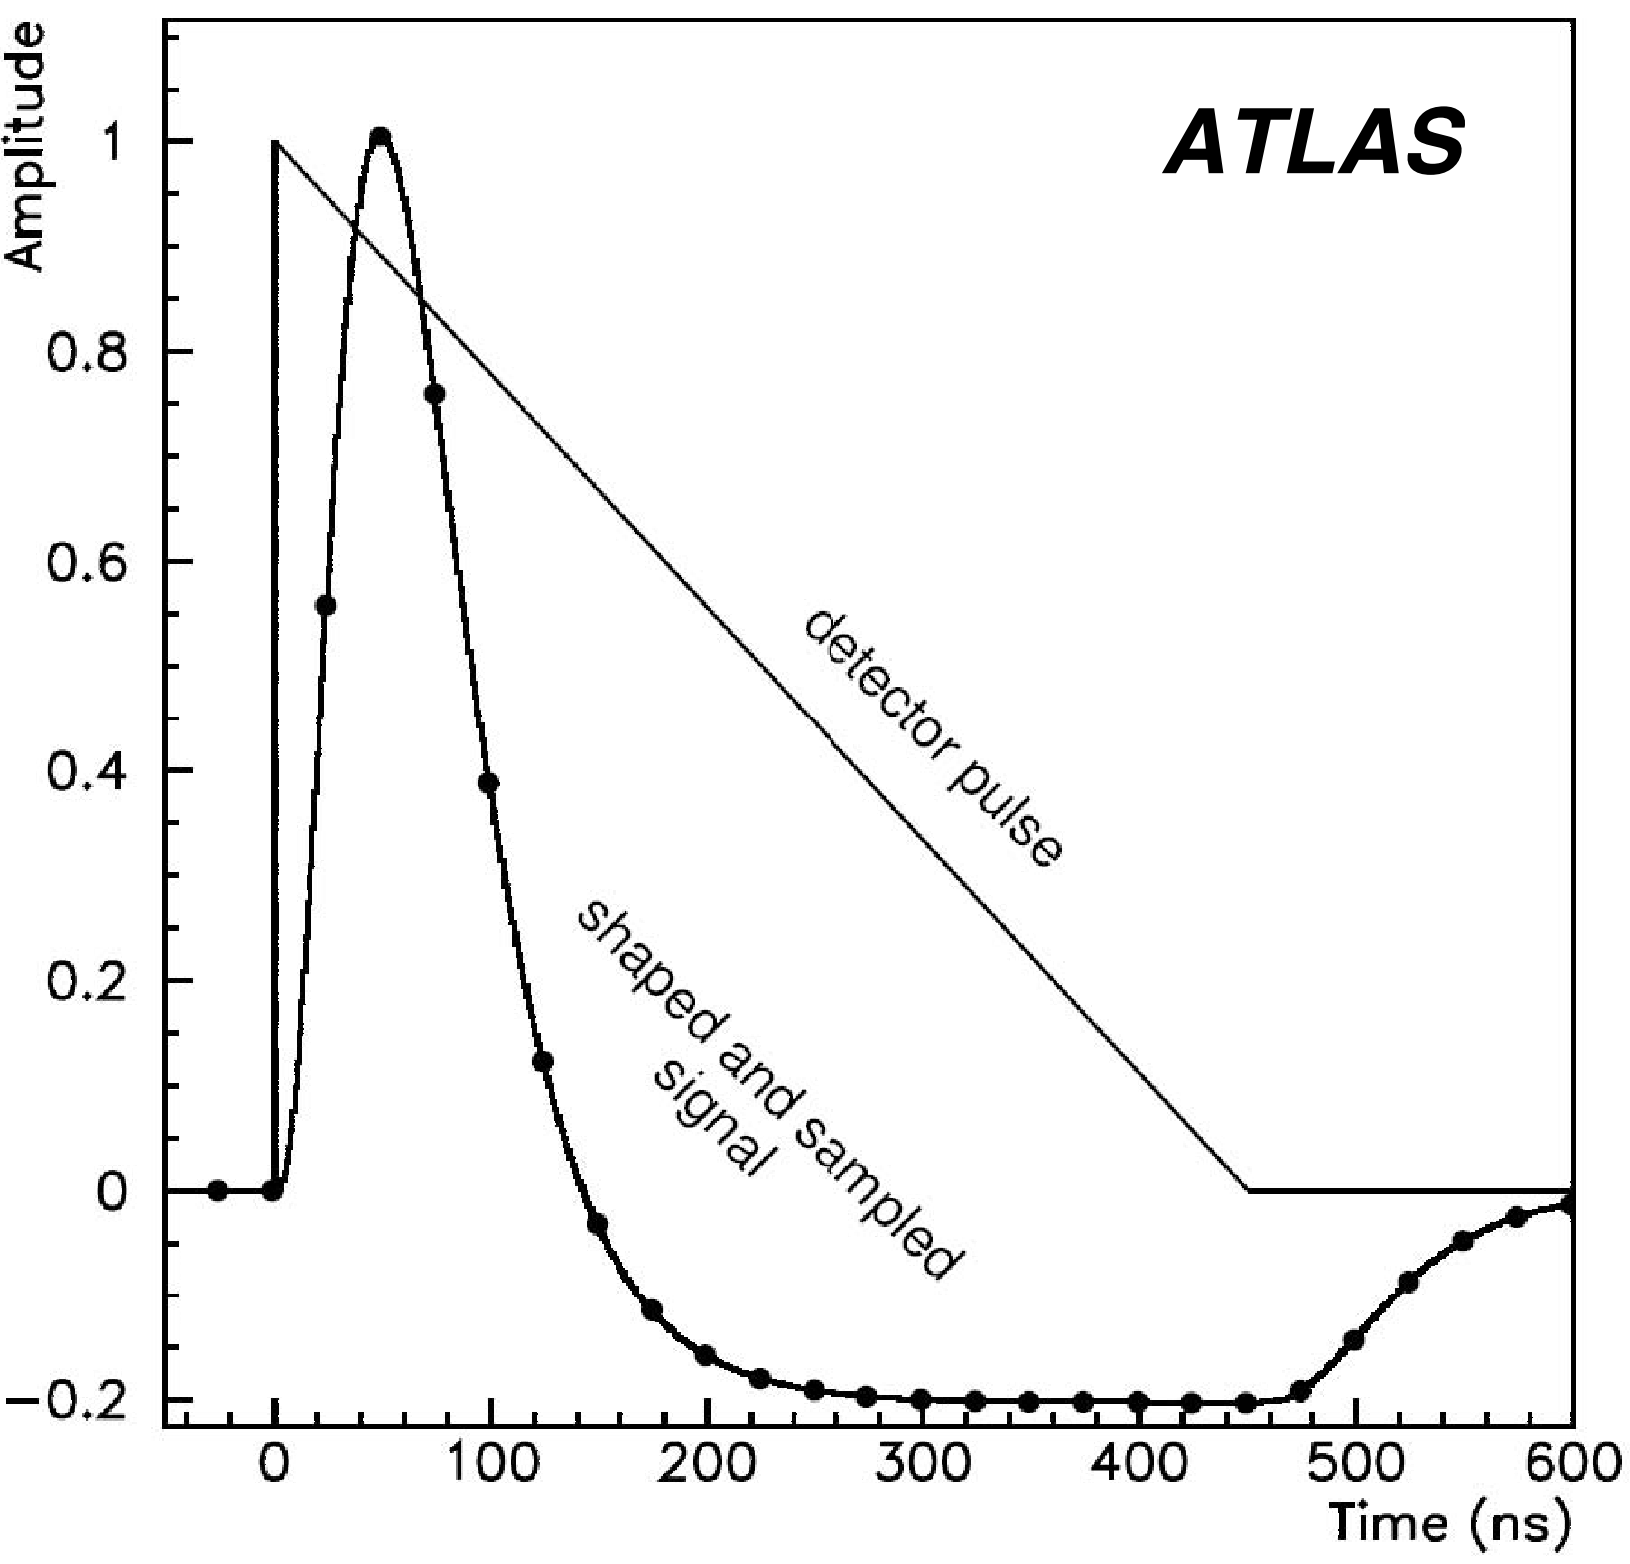
\includegraphics[width=0.5\linewidth]{tri_impulse.png}
    \caption{Форма импульса тока электромагнитного калориметра и выходного сигнала после формирования}
    \label{fig:tri_impulse}
\end{figure}
Электромагнитный калориметр имеет сложную геометрию в форме гармошки (аккордеон). Это позволяет достичь полной симметрии калориметра по азимутальному углу, а также обеспечить высокую гранулированность детектора и увеличить его быстродействие за счёт малого зазора между пластинами. Толщина EMB составляет более 24 радиационных длин ($X_0$, расстояние, на котором интенсивность потока электронов высокой энергии и гамма-излучения падает в e раз). Каждый модуль калориметра имеет ячеистую структуру и поделён на несколько слоёв по глубине, как, например, модуль центрального блока на рис. \ref{fig:em_cal_struct}. Калориметр сконструирован так, что наибольшая часть энергии собирается в среднем слое, задний слой собирает лишь хвост электромагнитного потока. Передний слой сегментирован таким образом, чтобы с его помощью можно было максимально точно определить направление падающих частиц. Исходя из этого, используя измерение энергии и положения всех ячеек в каждом слое калориметра можно восстановить энергию и траекторию рождённых частиц.
\begin{figure}[ht]
    \centering
    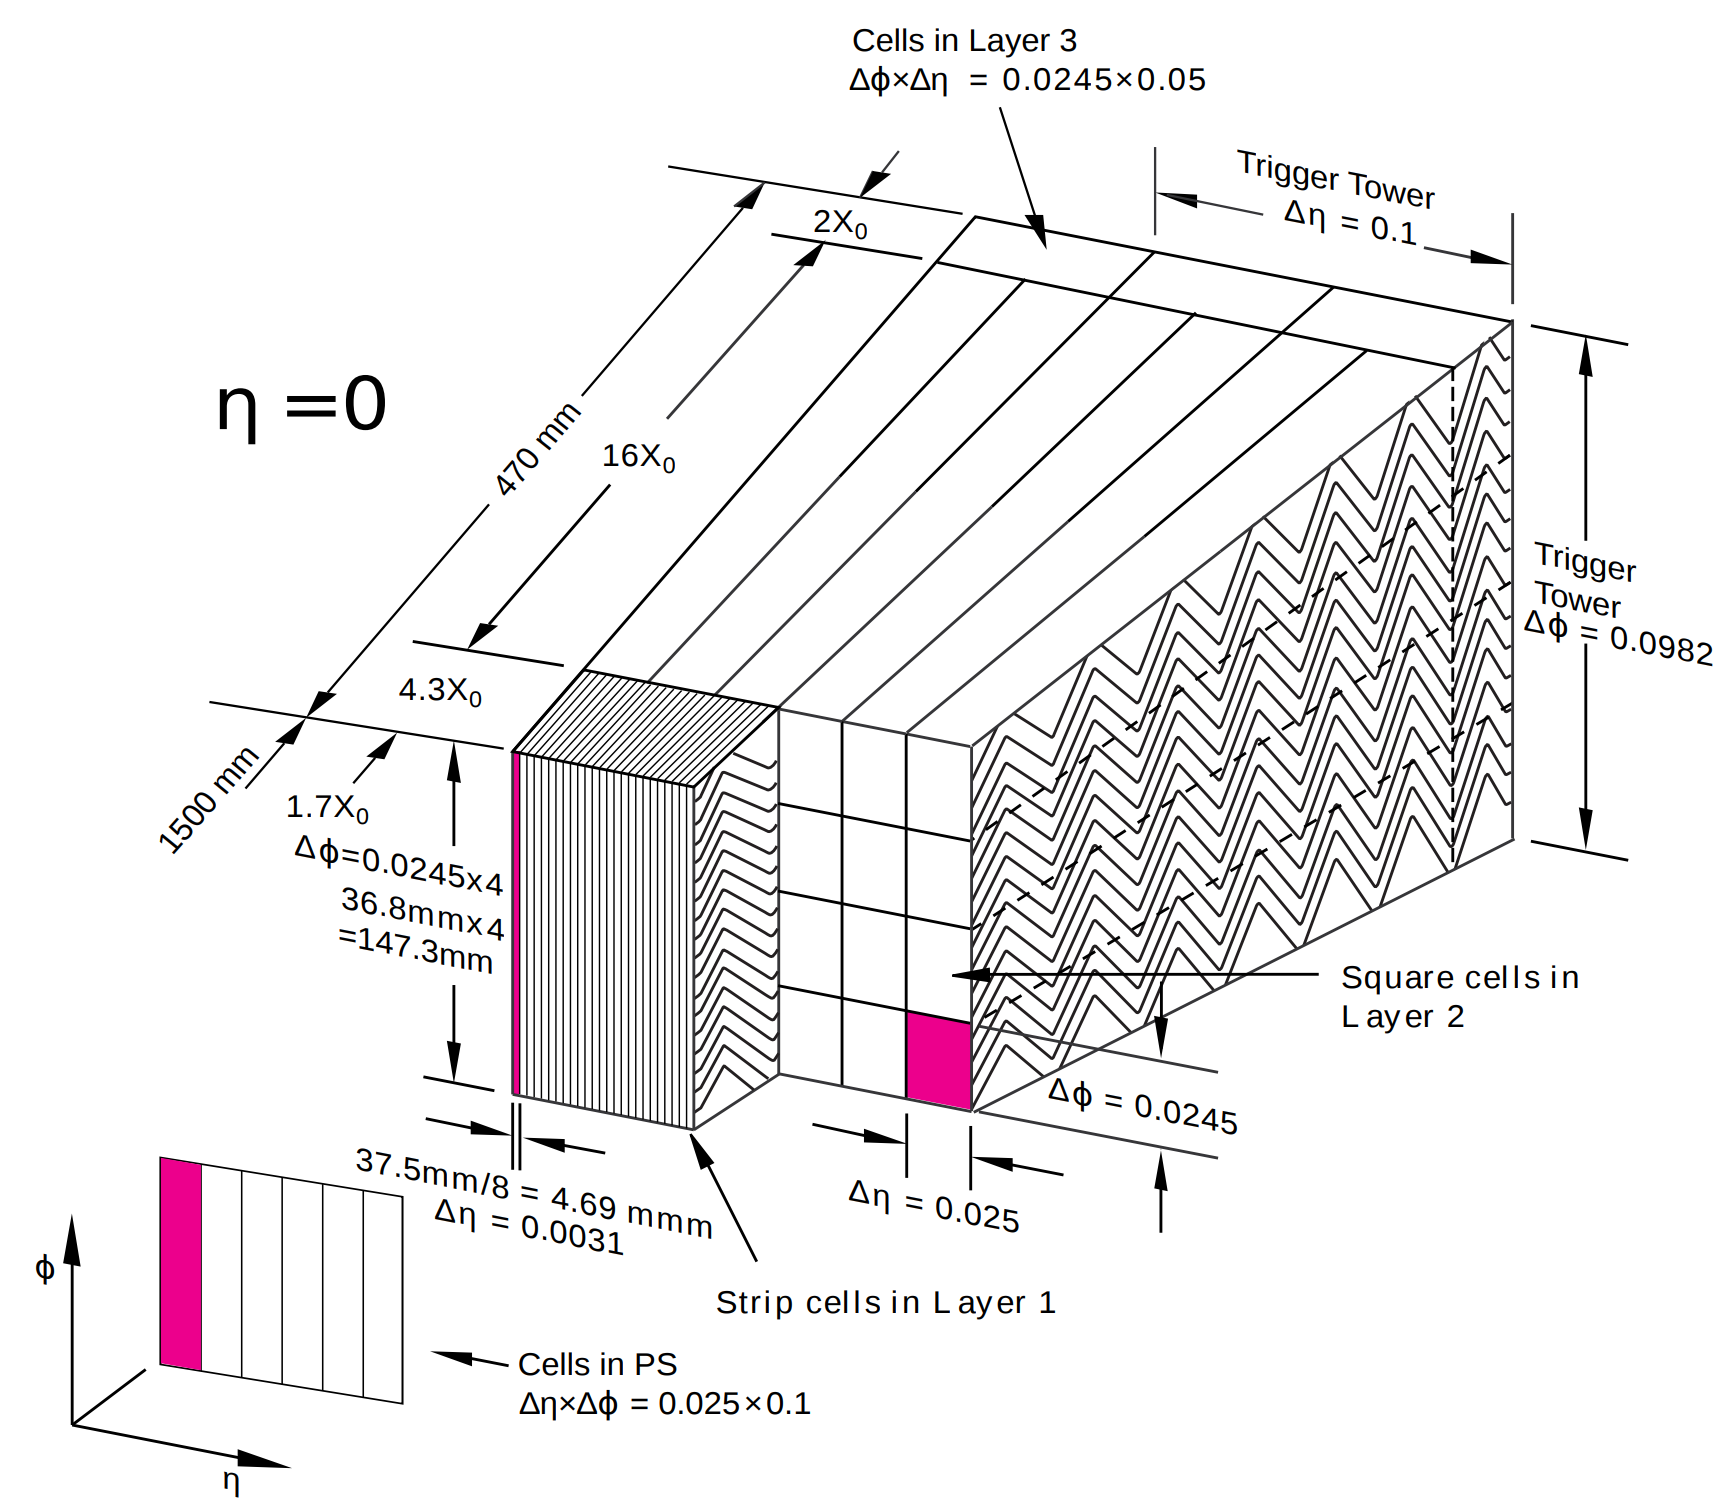
\includegraphics[width=0.7\linewidth]{em_cal_struct.png}
    \caption{Схема разделения модуля EMB по слоям}
    \label{fig:em_cal_struct}
\end{figure}


\subsubsection{Торцевой адронный калориметр}
Торцевой адронный калориметр(HEC -- hadronic end-cap) детектора ATLAS состоит из двух независимых колёс, которые установлены за блоками торцевого электромагнитного калориметра. Он обеспечивает адронное покрытие псевдобыстроты в диапазоне $1,5 < |\eta| < 3,2$. По принципу действия торцевой адронный калориметр похож на электромагнитный, но имеет плоскопараллельную структуру внутренней геометрии с медными пластинами-поглотителями, а в качестве адсорбера в нём используется железо.\par
Оба колеса калориметра состоят из 32 одинаковых по азимуту модулей. Переднее колесо разделено по глубине на две секции считывания, которые суммарно содержат 24 слоя поглотителя. Заднее колесо выполнено из 16 слоёв поглотителя, объединённых в один сегмент считывания. С каждой полученной ячейки регистрируется отдельный сигнал. Для обеспечения наилучшего отношения сигнала и шума предусилители считывающей электроники калориметра находятся в среде с низкой температурой и расположены по внешнему радиусу модулей.\par
Важным аспектом адронного калориметра является его способность обнаруживать мюоны, а также измерять их любые ионизационные потери и треки.\par


\subsubsection{Форвард калориметр}
Форвард калориметр находится ближе всего к пучку и обеспечивает электромагнитную и адронную калориметрию в диапазоне $3,2 < |\eta| < 4.9$. Из-за своего расположения он подвергается очень сильному воздействию дозы облучения мощностью до $10^6$ ${^\text{Гр}} / _\text{год}$ и потока нейтронов с кинетической энергией более 100 кэВ до 109 $\text{см}^{-2}\text{c}^{-1}$\parencite{tdr_old}. С учётом этих условий форвард калориметр разрабатывался с использованием следующих принципов:
\begin{itemize}
    \item механическая простота с применением небольшого набора материалов;
    \item использование радстойких материалов;
    \item использование материалов с высоким значением Z;
    \item достижение максимальной проективной толщины (вдоль проективных лучей от точки столкновения частиц);
    \item достижение максимальной средней плотности.
\end{itemize}\par
Калориметр состоит из трёх модулей: электромагнитного и двух адронных. В электромагнитной секции в качестве материала адсорбера используется медь, тогда как в адронных -- вольфрам. Номинальные внешние размеры у всех трёх модулей равные. Внутренняя структура представляет собой матрицу шестигранных трубок, расположенных вдоль пучка и изготовленных из материала поглотителя, в которые концентрично установлены медные электроды (рис. \ref{fig:f_cal_struct}). Пространство между стенками трубок и электродами заполнено жидким аргоном, выполняющим роль активного вещества. Конструкция позволяет точно контролировать зазор между электродами.
\begin{figure}[ht]
    \centering
    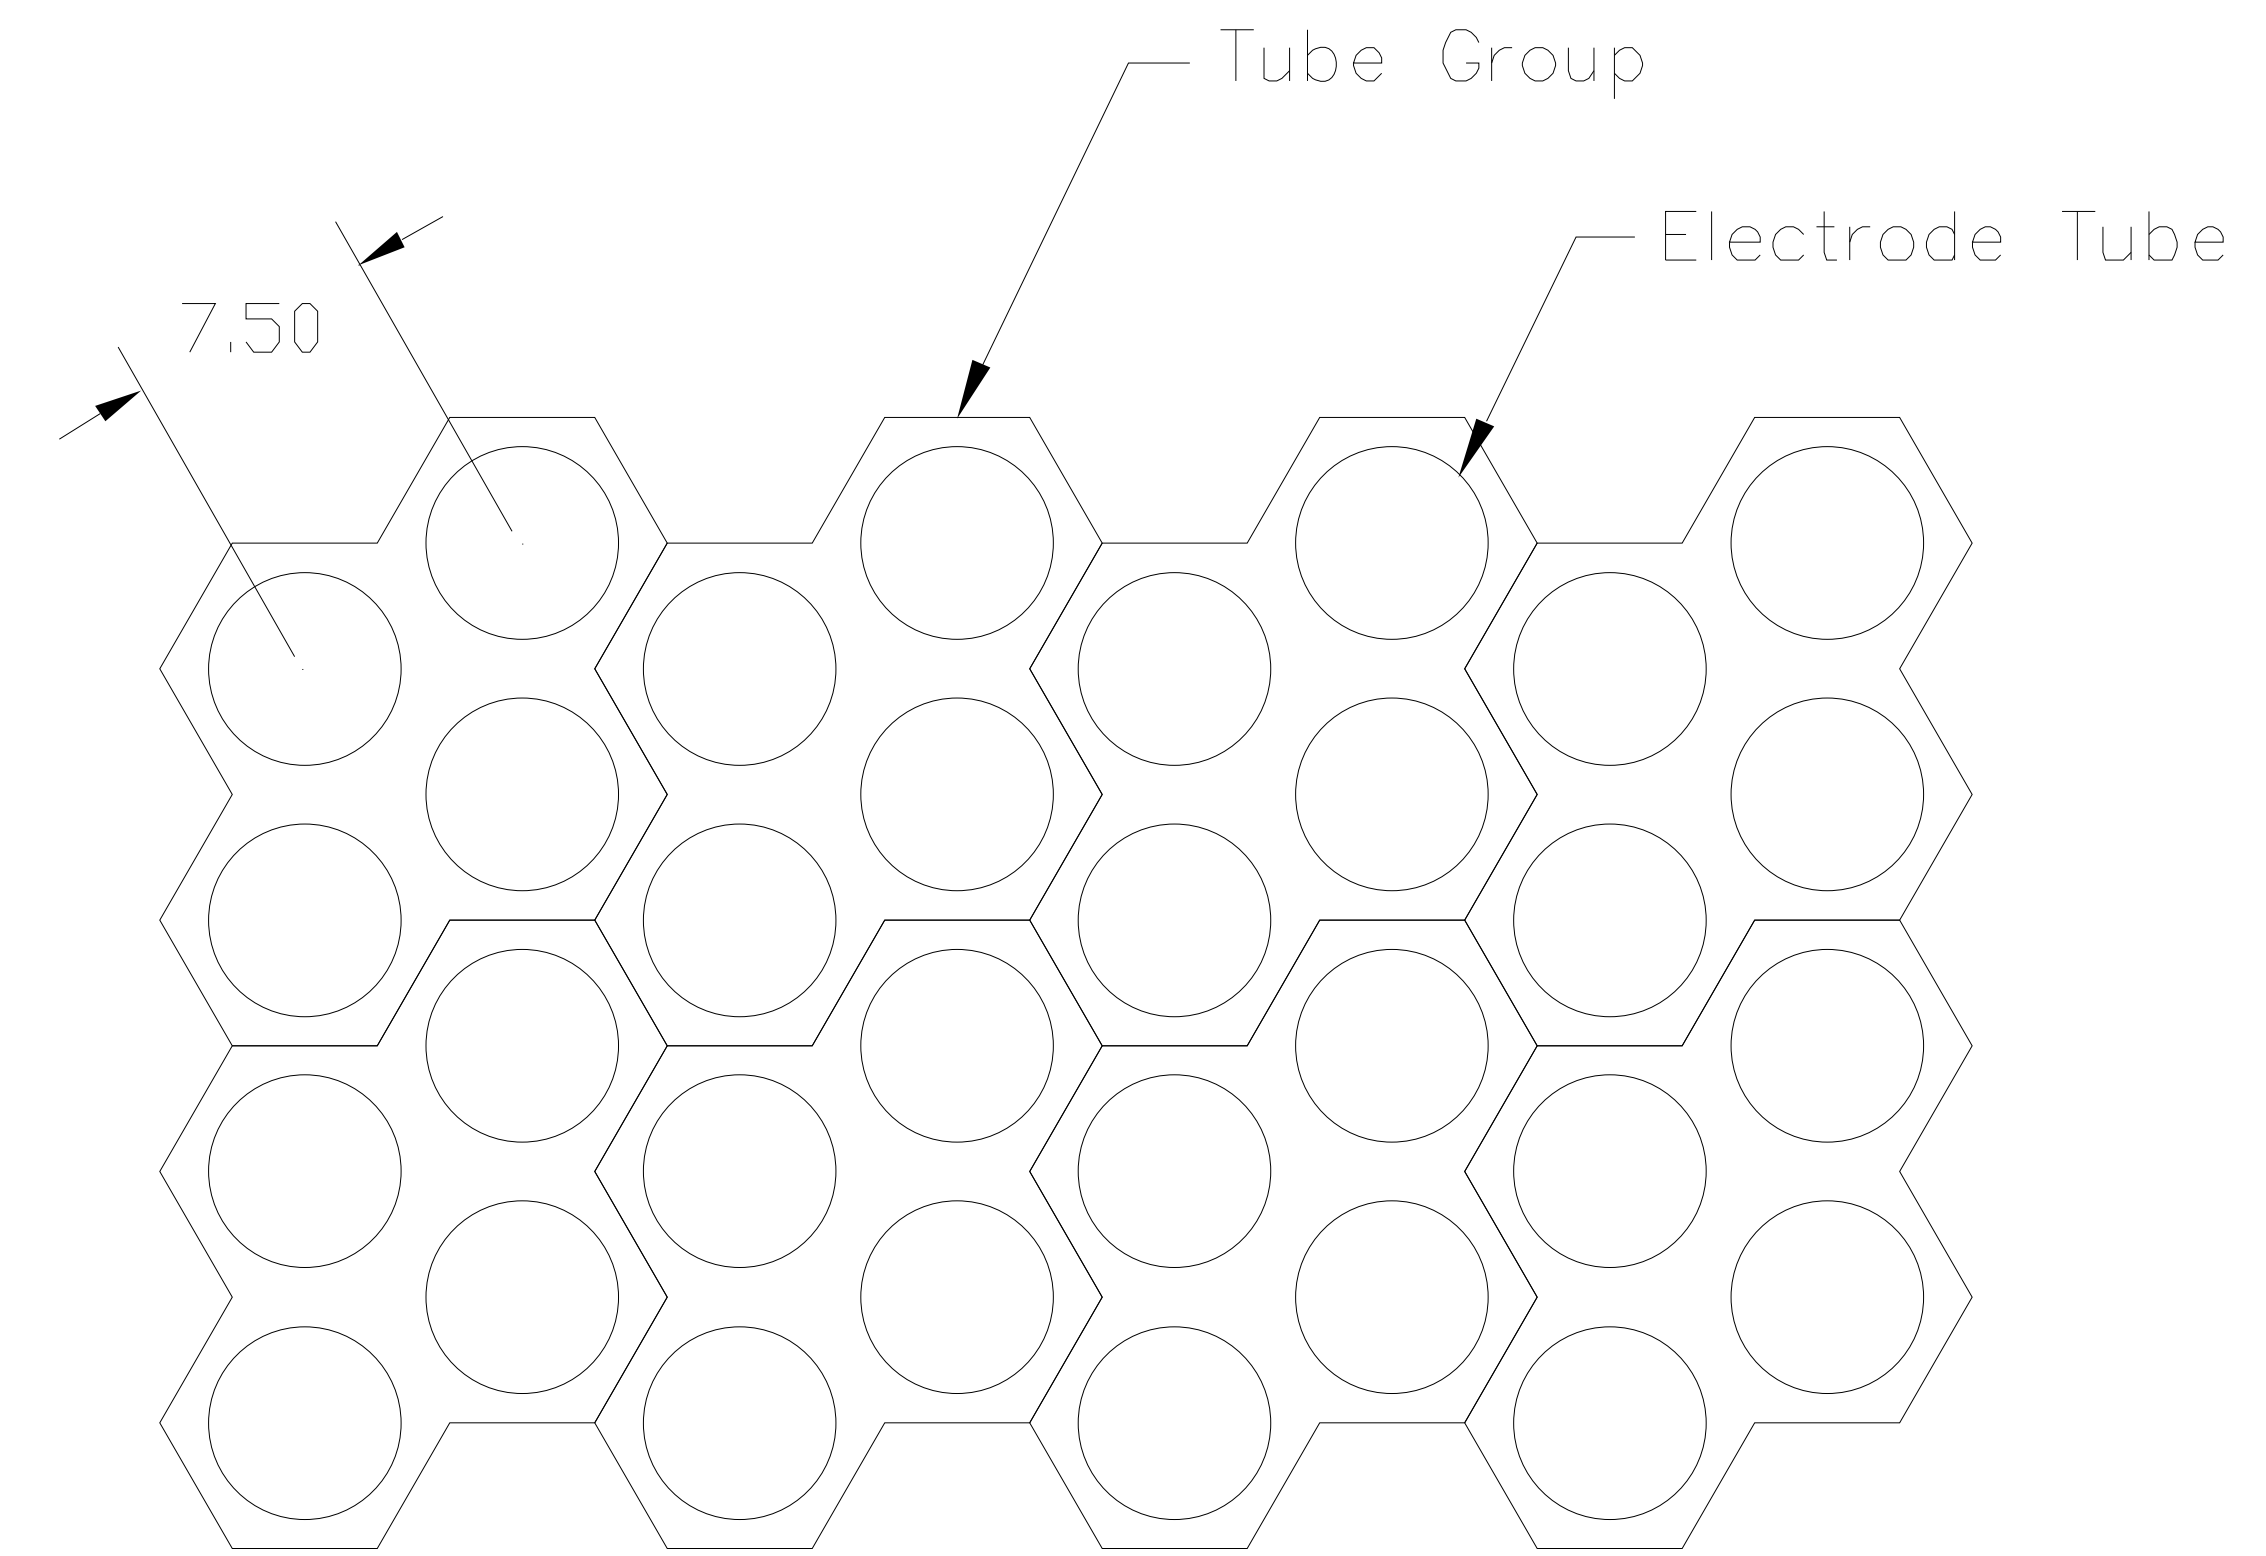
\includegraphics[width=0.6\linewidth]{f_cal_struct.png}
    \caption{Схема внутренней структуры форвард калориметра\parencite{tdr_old}}
    \label{fig:f_cal_struct}
\end{figure}\par
Таким образом, форвард калориметр способен работать в крайне радиационно нагруженных условиях, но при этом имеет сравнительно низкое разрешение. Однако, учитывая тот факт, что проходящие через него частицы имеют одни из наибольших абсолютных энергий, относительная точность остаётся достаточно высокой и такого разрешения вполне хватает для решения существующих физических задач.

